\scanpage{24}
\mspage{12}
\margin{23}

\figure{\begin{tikzpicture}[x=1cm,y=1cm]
\draw (-2.3,-.15)..controls(-1.2,.9)and(1.3,.8)..(2.4,-.35);
\draw (-2,.02)--(-2.05,.15) (-1.15,.48)--(-1.18,.61) (-.1,.56)--(-.12,.65);
\node[above]at(-2.05,.17){$x$};\node[above]at(-1.18,.62){$b$};\node[above]at(-.12,.66){$a$};
\end{tikzpicture}}

Si $b$ manque ds $\operatorname{Pol}^*(D)$, et sur l'arc $\overset{\frown}{ax}$ de $\operatorname{Pol}^*(D')$, ($x$ étant l'autre sommet de $\operatorname{Pol}^*(D')$ adjacent à $b$) on doit avoir
\[
\begin{aligned}
&\text{pondération de $\overset{\frown}{a,x}$ dans $\operatorname{Pol}^*(D)$}\\
&\qquad=\text{somme des pondérations de}\\
&\qquad\overset{\frown}{x,b},\ b,\ \overset{\frown}{b,a}\text{ dans }\operatorname{Pol}^*(D').
\end{aligned}
\]
[Pour exprimer commodément cette \unsure{égalité}, il faudrait développer la notion de pondération d'un sous-polygône d'un polygône pondéré, \deleted{\unsure{de}} de telle façon que les déploiements du polygône \inserted{pondéré} initial et du sous-polygône soient can. isom.]

La question se pose si les \deleted{\unsure{deux}} applications $\operatorname{Pol}^*(D)\mathbin{-}\operatorname{Pol}^*(D')$ peuvent se déduire des autres structures de $\Gamma^*(\underline\Sigma)$ (\deleted{\unsure{par structure}} cellularisation et \deleted{\unsure{la}} pondération).

Il faudrait d'abord passer en revue les \unsure{structures|structure} des \unsure{polygônes|polygône} $\operatorname{Pol}^*(D)$ (en d'abord $D$ non supercritique).

a) Parmi ses sommets, \deleted{il y a les} i.e. les arêtes de $\Gamma^*(\unsure{\underline\Sigma|D})$ en $D$, il y a les sommets de \uline{spécialisation} (arêtes \deleted{\unsure{entrantes}} \inserted{partant} de $D$), les arêtes de générisation (ce sont celles arrivant à $D$), et enfin les sommets neutres (arêtes libres en $D$, non-topologiques, arêtes dont l'autre extrémité est un ``bout'' au sens d'avant). Notons

a) L'ens des \deleted{arêtes} \inserted{sommets (ou arêtes)} de générisation est stable par l'antipodisme.

b) Si $a$ est une \deleted{arête} \inserted{sommet} de spécialisation, son antipodique n'est pas \deleted{arête} \inserted{sommet} de spécialisation.

c) Une \deleted{arête} \inserted{sommet} qui n'est ni \deleted{arête} de générisation, ni de spécialisation, ni antipodique d'une telle \inserted{(ou les deux)} est donc soit une ps. spécialisation, soit antipodique d'une telle, ce qui \unsure{implique} \inserted{au moins} qu'il est adjacent à un sommet de générisation, et la pondération de l'arête qui les joint est nulle, et réciproquement

\figure{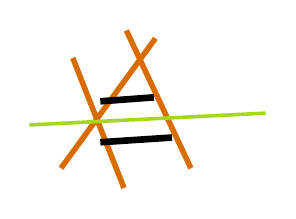
\begin{tikzpicture}[x=1cm,y=1cm]
\draw[orange!85!black,line width=2pt] (-.7,-.55)--(.5,1.1) (.1,-.8)--(-.55,.85) (.95,-.55)--(.13,1.2);
\draw[yellow!65!green,line width=1.3pt] (-1.1,0)--(1.9,.15);
\draw[black,line width=2.4pt] (-.2,.3)--(.48,.35) (-.2,-.22)--(.71,-.16);
\end{tikzpicture}}
